\documentclass[12pt]{article}
\usepackage{titling}
\usepackage[pdftex]{graphicx}
\usepackage[margin=1in]{geometry}
\linespread{1.3} %one-half spacing. 1.6 is double spaced. 
\frenchspacing
\usepackage{mathtools} %extra math symbols like arrows n shit
\usepackage[font=scriptsize]{caption}          %me being anal retentive about captions
\usepackage[raggedright]{sidecap}            %for side captions! Be aware, I don't think this is compatible with the float package...
		\sidecaptionvpos{figure}{c}        %centers captions vertically
\usepackage{gensymb}           %includes degree!
\usepackage{mhchem}        %There IS an easier way!
	%full isotope command: \ce{^{top#}_{bottom#}NameofElement^extraCrapAtTheEnd}  
	% ref: https://docs.moodle.org/27/en/Chemistry_notation_using_mhchem
\usepackage[font=scriptsize]{subcaption}  %because I just had to use a subcaption for one image. SIGH
\usepackage{simplewick}
\usepackage{amsmath}

\begin{document}


\section{Homework 1}

\subsection{Question 5}
$Q=M(\ce{^{223}_{88}Ra})-(M(\ce{^{14}_{6}C}+M(\ce{^{209}_{82}Pb})))=31.828$MeV

Then we can find the half-life from $T_{1/2}=\frac{\text{ln}2}{W P}$

with the decay rate defined as: 
 $W=\sqrt{\frac{Q}{2\mu R_t}}$ where $R_t$, the touching radius, is defined as $R_t=R_{decay product}+R_{daughter nucleus}$
 
 and the probability of decay defined as: 
 $P=$

Life tip: $e^2=1.44  \text{MeV}\cdot\text{fm}$


\newpage

\section{Project}
    
    \subsection{Part 1a}

Will type this later!

\subsection{Part 1b}
$H=H_0+H_1=
\begin{bmatrix}
	0 & 0\\
	0 & 2
	\end{bmatrix}
+
\begin{bmatrix}
	-g & -g \\
	-g & -g
	\end{bmatrix}
	=
\begin{bmatrix}
	-g & -g\\
	-g & 2-g\\
	\end{bmatrix}
	$
	\\
	\\
	Eigenvalues: 
	$1-g \pm \sqrt{g^2+1}$
	
	
\subsection{Part 1c: Hamiltonian Matrix}
No broken pairs, $S=0$, four lowest single particle levels filled by four particles. 

$H=H_0+H_1=\sum\limits_{p\sigma}  (p-1)a_{p\sigma}^\dagger a_{p\sigma} -g\sum\limits_{pq} P_{p}^{+}P_{q}^{-}$
\\
\\
$H_0=
\begin{bmatrix}
	2 & 0 & 0 & 0 & 0 & 0\\
	0 & 4 & 0 & 0 & 0 & 0 \\
	0 & 0 & 6 & 0 & 0 & 0\\
	0 & 0 & 0 & 6 & 0 & 0 \\
	0 & 0 & 0 & 0 & 8 & 0 \\
	0 & 0 & 0 & 0 & 0 & 10\\
\end{bmatrix}$
\\
\\
\\
$H_1=
\begin{bmatrix}
	-2g & -g & -g & -g & -g & 0\\
	-g & -2g & -g & -g & 0    & -g \\
	-g & -g & -2g & 0 & -g & -g\\
	-g & -g & 0 & -2g & -g & -g\\
	-g & 0 & -g & -g & -2g & -g\\
	0 & -g & -g & -g & -g & -2g\\
\end{bmatrix}$
\\
\\
\\
$H=H_0+H_1=
\begin{bmatrix}
	2-2g & -g & -g & -g & -g & 0\\
	-g & 4-2g & -g & -g & 0    & -g \\
	-g & -g & 6-2g & 0 & -g & -g\\
	-g & -g & 0 & 6-2g & -g & -g\\
	-g & 0 & -g & -g & 8-2g & -g\\
	0 & -g & -g & -g & -g & 10-2g\\
\end{bmatrix}$	



    
    
    
\newpage    
\section{Alex's email assignment from 7/7}
   Here's the interaction that goes with Gustav's talk today.

cceisdpn.int

You should use it with the sdpn.sp model space.

Before we meet at 2:30 your group should use this for our example of na23 and comment on

1) energy levels compared to exp

2) the extent to which isospin is conserved
    
    I put all this in the fridayex folder in rsh
    
\newpage




\section{NuShellX$^\copyright$ portion of project}

	\subsection{Comparison of \ce{^{18}O} and \ce{^{18}F} from NuShellX and our Shell model code}

Perfect match for oxygen isotopes

	\subsection{A lot of neutron-rich isotopes of Oxygen and Fluorine}

For USDB these agree quite well with the experimental results (when present) for a smaller sd-shell model. 



		\subsubsection{$^{30}$F in the pf-shell: woo hoo!}

This uses the ``sdpf" model space and the ``sdpfu" interaction, which happened to be the first interaction on the list in that model space. 

Without extreme truncation, this is so computationally intense that NuShellX can't even calculate how long it would take to run the program. 

\newpage
 
$^{30}F$ in the pf-shell: closed neutron shell with one neutron in the fp-shell to move about
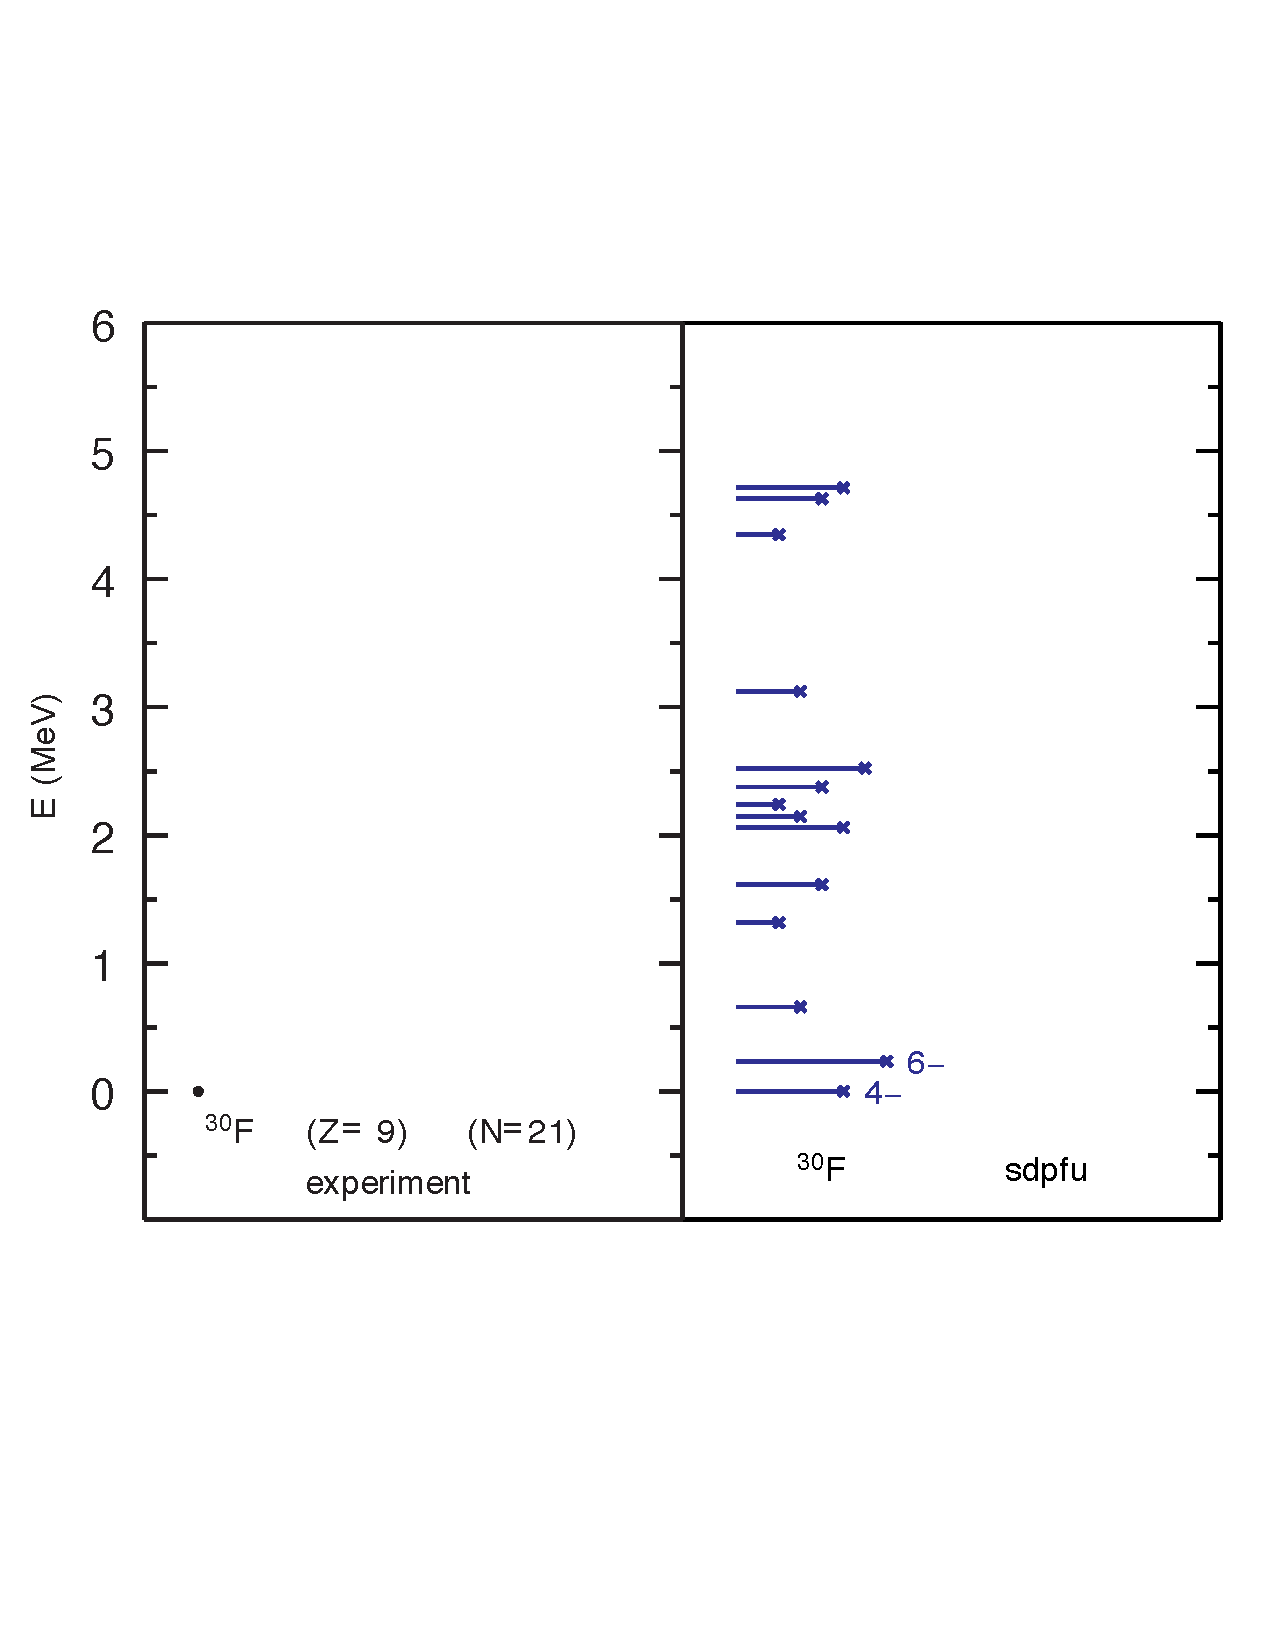
\includegraphics[width=\textwidth]{f_30u-1n.pdf}

\newpage

$^{30}$F in the pf-shell: 2 neutrons allowed in the fp-shell, 1 allowed out of the d3/2 shell

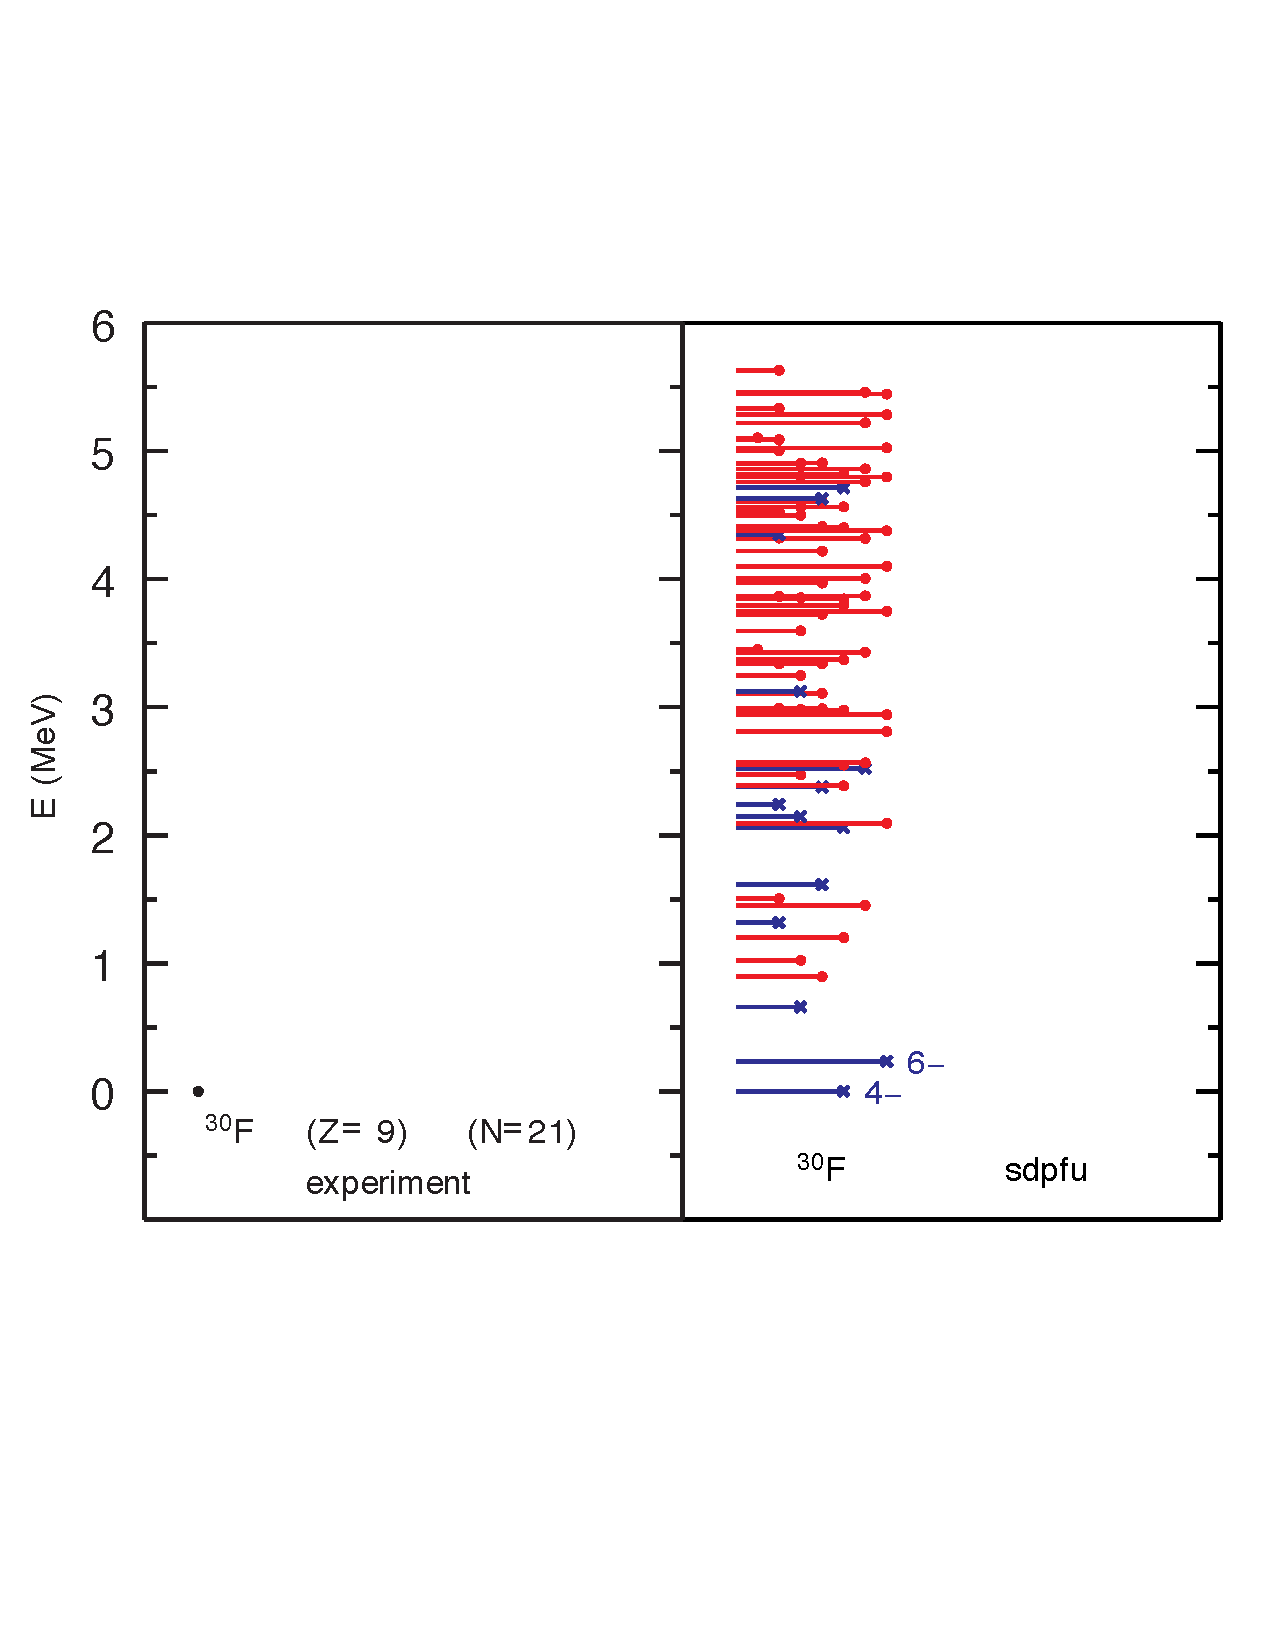
\includegraphics[width=\textwidth]{f_30u-2n.pdf} 
    
   \newpage
   
$^{30}$F in the pf-shell: 3 neutrons allowed in the fp-shell, 2 allowed out of the d3/2 shell

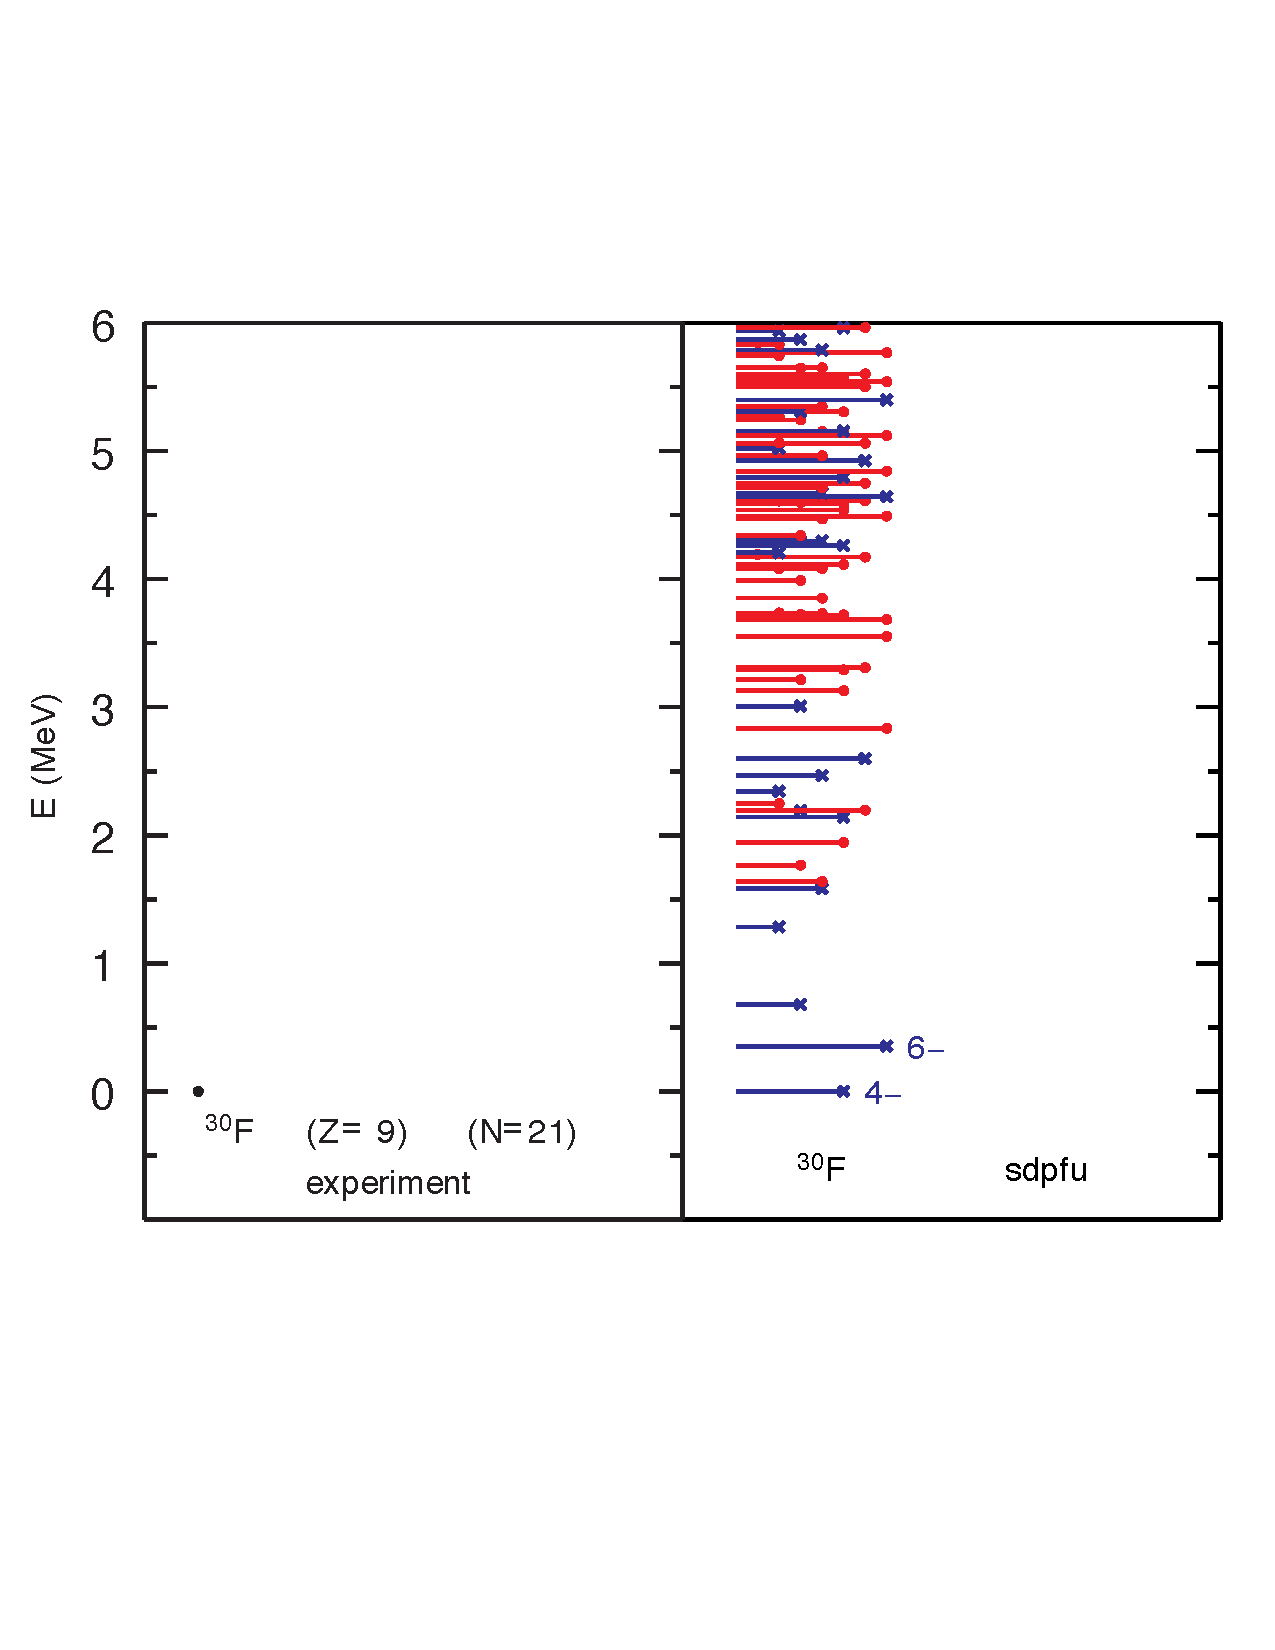
\includegraphics[width=\textwidth]{f_30u-3n.pdf}

\newpage

$^{30}$F in the pf-shell: all neutrons allowed out of the d3/2 shell into pf-shell

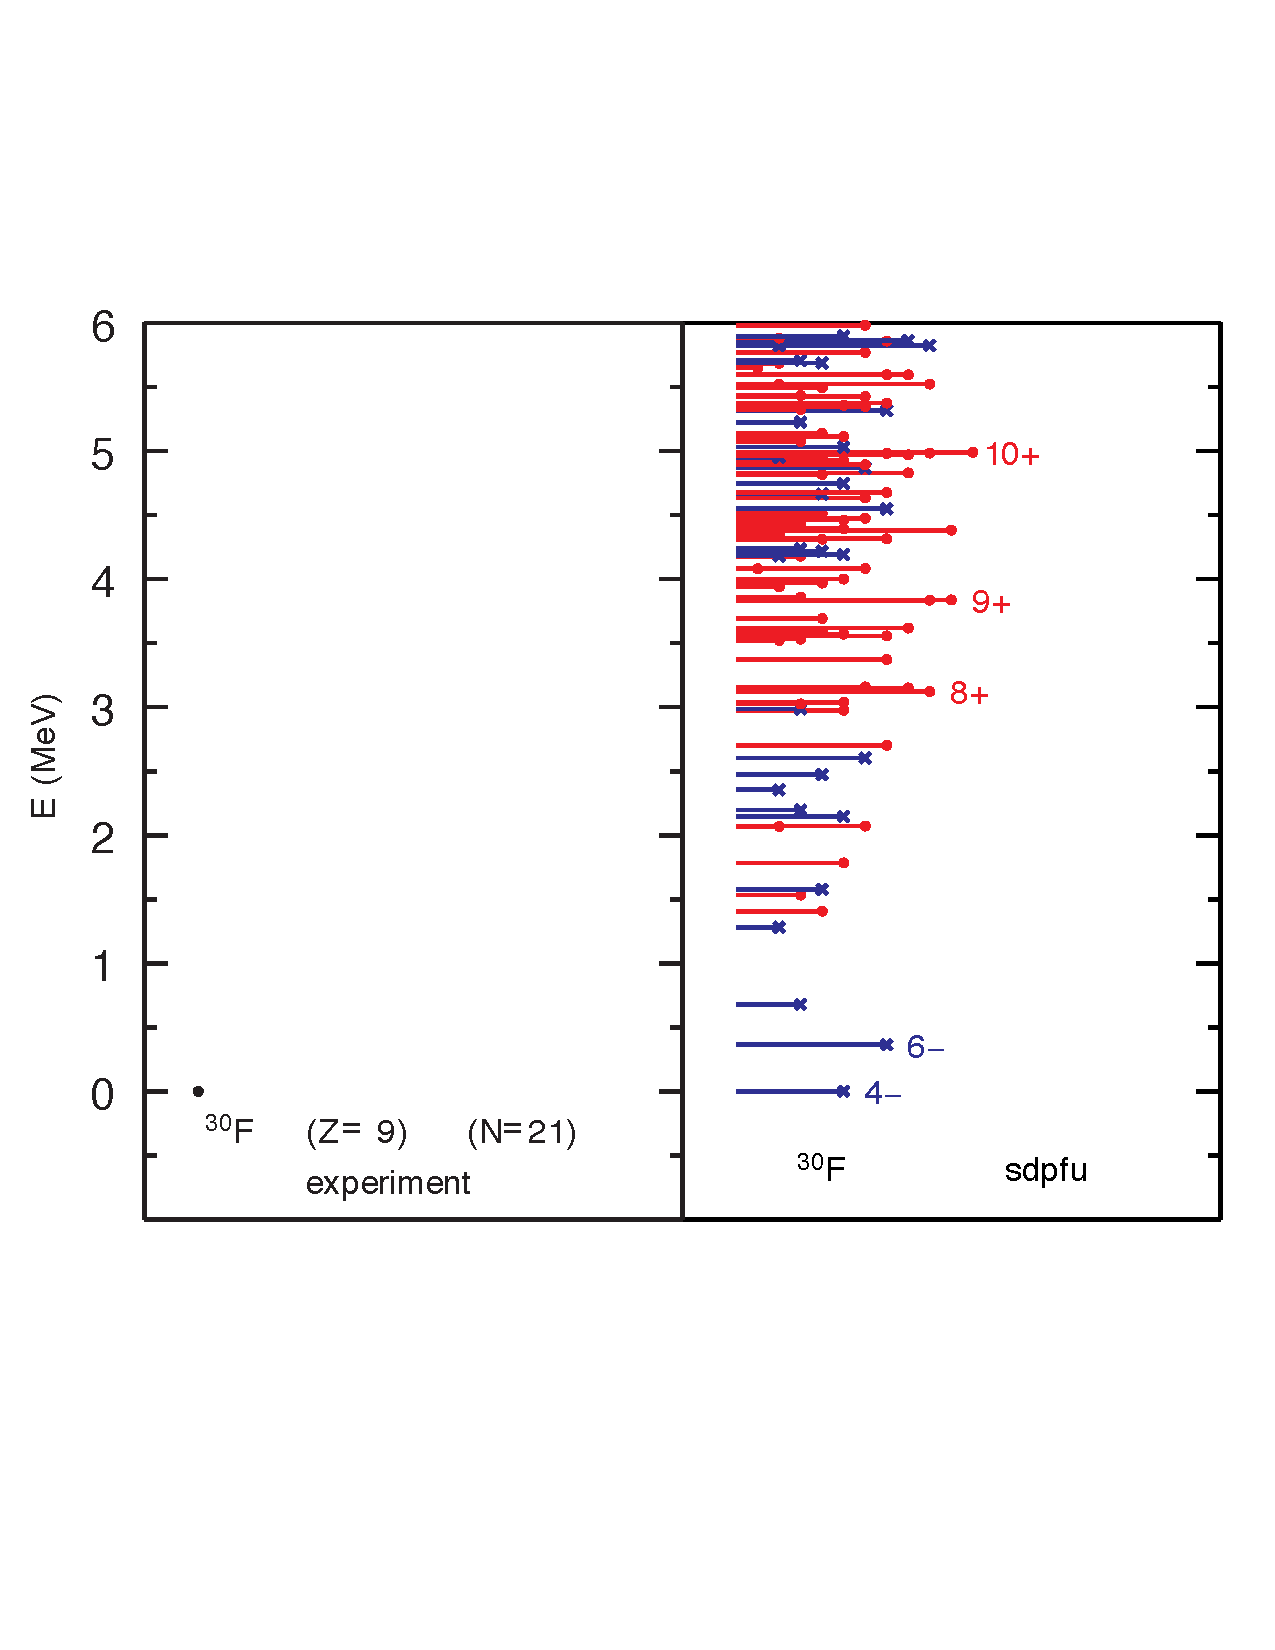
\includegraphics[width=\textwidth]{f_30u-allnfromd32.pdf}




	\subsection{Excited negative parity states in \ce{^{25}O} and \ce{^{25}F}?}
	
No, these do not exist because we are working in the sd-shell. 

	\subsection{Using monopole interactions to calculate the energies for the ground states of \ce{^{22-25}O} assuming a single Slater determinant for each. Compare the results of the last problem to the full sd model space results and experiment}
	
	\begin{center}
	\begin{tabular}{| l | c | r | r | r |}
	\hline
	   ... &\ce{^{22}O} & \ce{^{23}O} & \ce{^{24}O} & \ce{^{25}O} \\
	   \hline
	Previous problem &  & & & \\
	\hline
	Full sd model space (NuShellX) &  -32.429 MeV& -35.479 MeV  &  -40.088 MeV & -39.305 MeV  \\
	\hline
	Experiment & & & & \\
	\hline
\end{tabular}
\end{center}	




	\subsection{Some Spectroscopic Factors for Oxygen}
	\begin{figure}
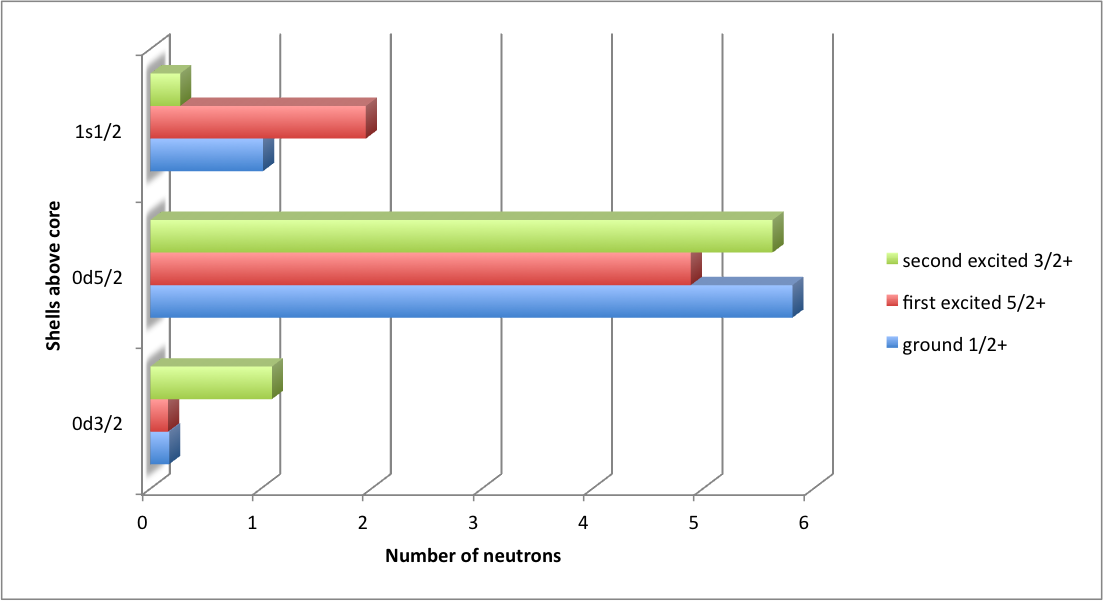
\includegraphics[width=\textwidth]{o23specs.png}
\caption{Oxygen 23 orbital occupations for the first 3 excited states from the *.occ file}
\end{figure}
		
		\subsubsection{Spectroscopic factors for  \ce{^{23}O^{gnd}} to \ce{^{22}O^{any state}}}

The total summed spectroscopic factor ($C^2S$)is 6.1420. The maximum SF should be 7. 

For the ground state we would expect (with an excess of 7 neutrons) for the 0d5/2 shell to be full and the 1s1/2 to have one neutron. 


		\begin{figure}
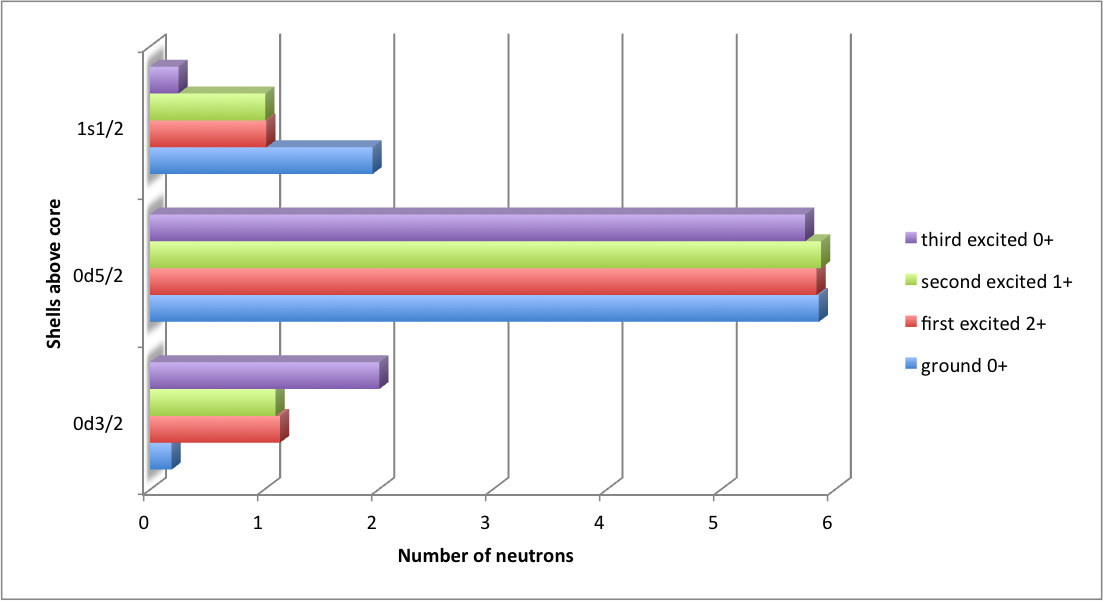
\includegraphics[width=\textwidth]{o24specs.png}
\caption{Oxygen 24 orbital occupations for the first 4 excited states from the *.occ file}
\end{figure}

		\subsubsection{Spectroscopic factors for  \ce{^{23}O^{gnd}} to \ce{^{24}O^{any state}}}
		
			\begin{center}
	\begin{tabular}{ r | l }
	State in \ce{^{24}O} & $(C^2S)$ \\
	\hline
	\hline
	0+  s1/2& 1.8587 \\
	1+  s1/2& 0.0342 \\
	1+  d3/2& 0.9391 \\
	2+  d3/2& 0.9671 \\
	2+  d5/2& 0.0476 \\
	3+ d5/2& 0.0206 \\
	\hline
	total sum & 3.8467\\
\end{tabular}
\end{center}




		\subsubsection{Spectroscopic factor for  \ce{^{23}O^{5/2+(1)}} to \ce{^{22}O^{0+(1)}}}
	
The calculated value is 0.590. It is small because this requires the neutron to carry away $J=5/2$ in angular momentum and corresponds to a less energetically favorable movement of particles among the orbitals. Starting with 2n in the 1s1/2 shell and 5n in the 2d5/2 shell, this particular decay would require the neutron to eject from the 0d5/2 shell and a drop of the neutron pair from the 1s1/2 orbital. The more energetically favorable ejection would just require the movement of both neutrons from the 1s1/2 orbital: one being ejected with $J=0$ and one dropping down into the 0d5/2 orbital. 

	\subsection{Use the interaction wspot to obtain the single particle decay width for the  \ce{^{23}O^{5/2+(1)}} state using the experimental neutron separation energy as a constraint. Combine this with the result of the last problem to obtain its neutron decay width and compare to experiment.}
	
The settings in the wspot *.dai file were: 
\begin{center}
 \begin{tabular}{l l l l l}
 22 & 8 & 1 & 0 & A, Z of target and A, Z of projectile\\
 0.04 & 0.04 & 0.1 & 5.0& $E_{min}, E_{max}, V_{min}, V_{max}$  \\
 0 & 2 & 5 & & Quantum numbers: n, l, m \\
 \end{tabular}
\end{center}
The energy values were chosen using the experimental value for the neutron separation energy for the 5/2+ level of \ce{^{23}O} was $S_n=40$ keV, and we used the spectroscopic factor $(C^2S)=0.0590$ calculated in the previous section. This converged to a value of $\Gamma_{s.p.}=0.1800$keV. Using the equation for neutron decay width: 
\begin{equation}
\Gamma_n=(C^2S)\Gamma_{s.p.}=(0.0590)(0.1800)=0.01062 \text{keV}=10.62 \text{eV}
\end{equation}
This agrees quite well with the experimental width of $\Gamma_n=10$eV. 

	\subsection{Calculate the neutron decay width of the  \ce{^{25}O^{3/2+(1)}} state and compare to experiment. Use the experimental neutron separation energy as a constraint.}

The settings in the wspot *.dai file were: 
\begin{center}
 \begin{tabular}{l l l l l}
 24 & 8 & 1 & 0 & A, Z of target and A, Z of projectile\\
 0.770 & 0.770 & 0.0 & 2.0& $E_{min}, E_{max}, V_{min}, V_{max}$  \\
 0 & 2 & 5 & & Quantum numbers: n, l, m \\
 \end{tabular}
\end{center}

Experimental neutron separation energy: $S_n=770$ keV

This converges to a value of $\Gamma_{s.p.}=138.6$ keV. 

Spectroscopic factors: from the USDB calculation in the article $(C^2S)=0.95$

\qquad From the usdb interaction from me using NuShellX: $(C^2S)=0.9721$


\begin{equation}
\Gamma_n=(C^2S)\Gamma_{s.p.}=(138.6)(0.9721)=137.733 \text{keV}
\end{equation}

The two different experimental values quoted in the same article for $\Gamma_n$ were 172 keV and 88 keV. We were right in the middle!




	\subsection{Calculate the gamma decay of \ce{^{22}O} for levels up to 6 MeV and compare to experiment. Calculate the B(E2) for Coulex to the $2^+$ state in \ce{^{22}O} and compare with experiment.}

	\subsection{Calculate the magnetic moment for the $1/2^+_1$ ground state of \ce{^{23}O} and compare to the single-particle (Schmidt) value}
	
	\subsection{Calculate the Fermi and Gamow-Teller $\beta$ decay of \ce{^{22}O}}



\end{document}